% !TeX root = RJwrapper.tex
\title{freesurfer: Connecting the Freesurfer Software with R}
\author{by John Muschelli, Elizabeth M. Sweeney, Ciprian M. Crainiceanu}

\maketitle

\abstract{%
We present the package \CRANpkg{freesurfer}, a set of R functions that
interface with Freesurfer, a commonly-used open-source software package
for processing and analyzing structural neuroimaging data, specifically
T1-weighted images. The \pkg{freesurfer} package performs operations on
\code{nifti} image objects in R using command-line functions from
Freesurfer, and returns R objects back to the user. \pkg{freesurfer}
allows users to process neuroanatomical images and provides
functionality to convert and read the output of the Freesurfer pipelines
more easily, including brain images, brain surfaces, and Freesurfer
output tables.
}

\begin{Schunk}
\begin{Soutput}
#> Warning: package 'knitr' was built under R version 3.3.2
\end{Soutput}
\end{Schunk}

\section{Introduction}\label{introduction}

\label{sec:intro}

Freesurfer is a commonly-used software for processing and analyzing
anatomical neuroimaging data \citep{fischl2012freesurfer}, developed by
the Laboratory for Computational Neuroimaging at the Athinoula A.
Martinos Center for Biomedical Imaging. This software provides
open-source, command-line tools for image processing tasks such as brain
extraction/skull-stripping \citep{segonne2004hybrid}, bias-field
correction \citep{sled_nonparametric_1998}, segmentation of structures
within the brain \citep{fischl2002whole,fischl2004sequence}, and image
registration \citep{fischl1999high,reuter2010highly}. In addition to
these functions, Freesurfer has functions that perform fully-automated
pipelines for the user.

While there exist a number of R packages for reading and manipulating
image data, including \CRANpkg{AnalyzeFMRI}
\citep{bordier_temporal_2011} and \CRANpkg{fmri}
\citep{tabelow_statistical_2011}, which analyze functional magnetic
resonance images (MRI) and perform spatial smoothing,\CRANpkg{RNiftyReg}
\citep{modat_rniftyreg:_2013}, which performs image registration, and
\CRANpkg{dpmixsim} \citep{dpmixsim} and \CRANpkg{mritc} \citep{mritc},
which perform image clustering and segmentation (see the Medical Imaging
CRAN task view
\url{http://cran.r-project.org/web/views/MedicalImaging.html} for more
information). These packages are useful for performing image analysis,
but the neuroimaging community has tools that functions to perform
specific analyses, which have been used before by other users.
Freesurfer provides methods that not currently implemented in R,
including surface-based registration and completely automated image
segmentation pipelines. The \pkg{ANTsR} package
(\url{https://github.com/stnava/ANTsR}) is a currently unpublished R
package where additional image analysis functionality has been
implemented, but not including all the functionality Freesurfer has.
Moreover, having multiple options for image processing through R enables
users to compare methods and provides the flexibility of using multiple
packages to achieve a working data processing pipeline.

We provide an interface to users to the state-of-the-art anatomical
processing implemented in Freesurfer, as well as a suite of tools that
simplify analyzing the output of Freesurfer. The \pkg{freesurfer}
package allows R users to perform a complete anatomical imaging analyses
without necessarily learning Freesurfer-specific syntax, while keeping
both the image processing and analysis within R.

\subsection{R function setup}\label{r-function-setup}

To use \pkg{freesurfer}, a working installation of Freesurfer is
required (downloads available:
\url{http://freesurfer.net/fswiki/DownloadAndInstall}). The following
code was run using Freesurfer version
``freesurfer-Darwin-lion-stable-pub-v5.3.0''. The Freesurfer version can
be accessed using the \pkg{freesurfer} \code{fs\_version} function. The
path of Freesurfer must also be set. When using R from a shell
environment, after the \code{FREESURFER\_HOME} environment variable is
set (which is done when installing Freesurfer), \pkg{freesurfer} will
use this as the path to Freesurfer. If using R through a graphical user
interface (GUI) such as RStudio (RStudio, Boston, MA), environmental
variables and paths are not explicitly exported. Therefore,
\code{FREESURFER\_HOME} is not set and \pkg{freesurfer} will try the
default directories of Mac OSX and Linux. Freesurfer is only available
on Windows via a virtual machine. If the user did not perform an
standard installation of Freesurfer, the path to Freesurfer can be
specified using \code{options(freesurfer.path="/path/to/freesurfer")}.
The \code{have\_fs} function tests whether a user has a Freesurfer
installation, returning a logical, which is useful for \code{if}
statements within examples. If \code{have\_fs} function returns is
\code{TRUE}, the \code{fs\_dir} function will return the directory of
the Freesurfer installation.

\subsubsection{Structure of Freesurfer
analyses}\label{structure-of-freesurfer-analyses}

During the installation of Freesurfer, environment variables in addition
to \code{FREESURFER\_HOME} are set. One of these variables is
\code{SUBJECTS\_DIR}, which refers to a directory of the output of
analysis from all subjects. The \code{fs\_subj\_dir} function will
return the path to the Freesurfer subjects directory if it is set. This
default setup of a subjects directory in Freesurfer allows users to
simply specify a subject identifier to analyze, rather than a specific
path or multiple intermediate files.

This setup may not be desirable if the user prefers to structure his or
her data differently. For example, if data from multiple studies are
present, these may be organized into different folders in different
locations. Some functions in Freesurfer rely on the \code{SUBJECTS\_DIR}
variable to run. These functions take the subject name as the main
argument rather than a file, which is more common. To provide
flexibility to the user, \pkg{freesurfer} allows most functions to
specify a file or different directory rather than specifying the
subject.

One example is the \code{asegstats2table} Freesurfer function.
Freesurfer performs segmentations of the anaomtical image into different
stuctures and has associated statistics for each region such as volume
and mean intensity. The \code{asegstats2table} function transforms
\textbf{a}natomical \textbf{seg}mentation \textbf{stat}istics from into
to a table. The default argument for \code{asegstats2table} is to pass
in a subject name rather than a file. The \pkg{freesurfer}
\code{asegstats2table} function allows the R user to specify the subject
name, but also allows the user to alternatively specify a filename
instead. This function will temporarily set \code{SUBJECTS\_DIR} to a
temporary directory, copy the file to that directory, execute the
command, then reset the \code{SUBJECTS\_DIR} variable. This provides a
more flexible workflow, while not overriding the default directory set
in \code{SUBJECTS\_DIR}. This functionality allows users to have
separate folders with subjects and read in the data by simply switching
the \code{subj\_dir} argument in the R function.

\subsection{Reconstruction pipeline in
Freesurfer}\label{reconstruction-pipeline-in-freesurfer}

The Freesurfer pipeline and analysis workflow for neuroanatomical images
is designed to work with T1-weighted structural MRI of the brain. The
full pipeline is implemented in the Freesurfer \code{recon-all}
function, where the ``recon'' stands for reconstruction
(\url{https://surfer.nmr.mgh.harvard.edu/fswiki/recon-all}). The
\texttt{recon-all} function is the main workhorse of Freesurfer and is
the most commonly used. Using the \code{-all} flag in the the
\code{recon-all} function performs over 30 different steps and takes
20-40 hours to fully process a subject
(\url{https://surfer.nmr.mgh.harvard.edu/fswiki/recon-all}). This
process is the recommended way of fully processing an T1-weighted image
in Freesurfer, and is implemented in the \texttt{recon\_all}
\pkg{freesurfer} function.

In the \texttt{recon\_all} function, users must specify the input file
(a T1-weighted image), the output directory (if different than
\code{SUBJECTS\_DIR}), and the subject identifier. The results will be
written in the individual subject directory, a sub-directory of
\code{SUBJECTS\_DIR}. The syntax is:

\begin{Schunk}
\begin{Sinput}
recon_all(infile, outdir, subjid)
\end{Sinput}
\end{Schunk}

If there are problems with the result of this processing, there are
multiple steps where users can edit certain parts of the processing,
such as brain extraction, where non-brain tissues are removed from the
image. The remainder of the pipeline can be run after these steps are
corrected. The full pipeline is broken down into 3 separate sets of
steps, referred to as \code{autorecon1}, \code{autorecon2}, and
\code{autorecon3}, which correspond to the same-named flags in
\code{recon-all} used to initiate these steps. We have written wrapper
functions \code{autorecon1}, \code{autorecon2}, and \code{autorecon3},
respectively, so users can run pieces of the pipeline if desired or
restart a failed process after correction to the data.

\subsection{\texorpdfstring{Imaging formats in \pkg{freesurfer} and
R}{Imaging formats in  and R}}\label{imaging-formats-in-and-r}

The \CRANpkg{freesurfer} package relies on the \CRANpkg{oro.nifti}
\citep{whitcher_working_2011} package implementation of images (referred
to as \code{nifti} objects) that are in the Neuroimaging Informatics
Technology Initiative (NIfTI) format. For Freesurfer functions requires
an image, the R \pkg{freesurfer} functions that call those Freesurfer
functions will take in a file name or a \code{nifti} object. The R code
will convert the \code{nifti} to the corresponding input required for
Freesurfer. From the user's perspective, the input/output process is all
within R, with one object format (\code{nifti}). The advantage of this
approach is that the user can read in an image, do manipulations of the
\code{nifti} object using standard syntax for arrays, and pass this
object into the \pkg{freesurfer} R function. Thus, users can use R
functionality to manipulate objects while seamlessly passing these
object to Freesurfer through \pkg{freesurfer}.

Other Freesurfer functions require imaging formats other than NIfTI,
such as the Medical Imaging NetCDF (MINC) format
(\url{http://www.bic.mni.mcgill.ca/ServicesSoftware/MINC}). The
Freesurfer installation provides functions to convert from MINC to NIfTI
formats and there are implemented in functions such as \code{nii2mnc}
and \code{mnc2nii} in R. Moreover, the \code{mri\_convert} Freesurfer
function has been interfaced in \pkg{freesurfer} (same function name),
which allows for a more general conversion tool of imaging types for R
users than currently implemented in native R. Thus, many formats can be
converted to NIfTI and then read into R using the \code{readNIfTI}
function from \pkg{oro.nifti}.

\section{Example analyses and use of
functions}\label{example-analyses-and-use-of-functions}

\subsection{Reconstruction}\label{reconstruction}

For this paper, we will not run the analysis on a subject, but rather
explore the output results for a subject included in the Freesurfer
installation for reproducibility for the user. In particular, in the
default Freesurfer subjects directory, there is a subject named
``bert''. If we were to run all the analyses, we would use the
\code{recon\_all} code (described below):

\begin{Schunk}
\begin{Sinput}
recon_all(infile = "/path/to/T1.nii", subjid = "bert")
\end{Sinput}
\end{Schunk}

We see the result of this output in the ``bert'' directory, which
includes a series of sub-directories:

\begin{Schunk}
\begin{Sinput}
list.files(path  = file.path(fs_subj_dir(), "bert"))
\end{Sinput}
\begin{Soutput}
 [1] "bem"     "label"   "mri"     "scripts" "src"     "stats"   "surf"   
 [8] "tmp"     "touch"   "trash"  
\end{Soutput}
\end{Schunk}

We will explore the results in ``mri'', which contain imaging data,
``stats'', which containing statistics based on structures of the brain,
and ``surf'', which contain the surface and curvature output from the
Freesurfer processing.

\subsection{\texorpdfstring{MRI conversion: the \code{mri\_convert}
function}{MRI conversion: the  function}}\label{mri-conversion-the-function}

The typical output format of brain volumes from Freesurfer is MGH/MGZ
format, which is explained here:
\url{https://surfer.nmr.mgh.harvard.edu/fswiki/FsTutorial/MghFormat}. As
NIfTI formats are one of the most common formats and has been the common
format for analysis in the \pkg{oro.nifti} and \CRANpkg{neurobase}
packages, it is useful to convert these files to a NIfTI format to read
into R. The \code{mri\_convert} Freesurfer function will be used for
that conversion. Here we will use the T1-weighted image from the
``bert'' subject and convert it to NIfTI, and read it into R:

\begin{Schunk}
\begin{Sinput}
library(freesurfer)
bert_dir = file.path(fs_subj_dir(), "bert") # subject directory
t1_mgz = file.path(bert_dir, "mri", "T1.mgz") # mgz file
t1_nii_fname = tempfile(fileext = ".nii.gz") # temporary NIfTI file
freesurfer::mri_convert(t1_mgz, t1_nii_fname) # conversion
img = neurobase::readnii(t1_nii_fname) # read in outputs
\end{Sinput}
\end{Schunk}

As this is a commonly-used process, we have wrapped these two steps into
the \texttt{readmgz} and \texttt{readmgh} functions, which combine the
\texttt{mri\_convert} and \texttt{readnii} functions. Here we show that
these steps are equivalent to the \texttt{readmgz} function:

\begin{Schunk}
\begin{Sinput}
img_mgz = readmgz(t1_mgz)
identical(img, img_mgz)
\end{Sinput}
\begin{Soutput}
[1] TRUE
\end{Soutput}
\end{Schunk}

Now that we have the image in R, we can plot it using the standard
plotting tools for \texttt{nifti} objects:

\begin{Schunk}
\begin{Sinput}
neurobase::ortho2(img, add.orient = FALSE, mask = img > 40)
\end{Sinput}
\begin{figure}
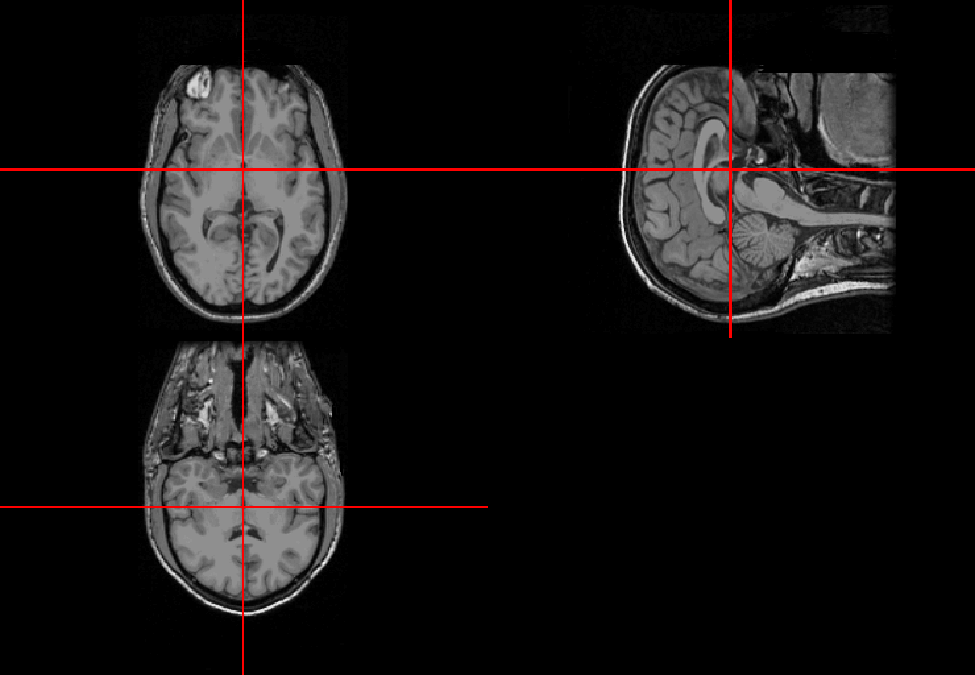
\includegraphics{Freesurfer_files/figure-latex/mri_plot-1} \caption[Plot of T1-weighted image from bert subject in Freesurfer]{Plot of T1-weighted image from bert subject in Freesurfer.}\label{fig:mri_plot}
\end{figure}
\end{Schunk}

The result is in figure \ref{fig:mri_plot}, which contains 3 slices of
the head: axially, viewing the brain from the top of the head (top
left), sagittally, viewing the brain from the right side (top right) and
coronally, viewing the brain from the back of the head (bottom left).

Note, the image is not stored in the right/posterior/inferior (RPI)
orientation which is assumed when displaying using the \pkg{neurobase}
\code{ortho2} function
\url{http://www.grahamwideman.com/gw/brain/orientation/orientterms.htm}.
We can use the \texttt{rpi\_orient} function in \CRANpkg{fslr} (version
\(\geq\) 2.4.0) \citep{muschelli2015fslr} or \texttt{fslswapdim} to
reorient the image to the assumed orientation.

\begin{Schunk}
\begin{Sinput}
L = fslr::rpi_orient(img)
reoriented_img = L[["img"]]
\end{Sinput}
\end{Schunk}

We see that this function puts this image in the RPI orientation, which
matches the assumed orientation for \texttt{ortho2}:

\begin{Schunk}
\begin{Sinput}
neurobase::ortho2(reoriented_img, mask = reoriented_img > 40)
\end{Sinput}
\begin{figure}
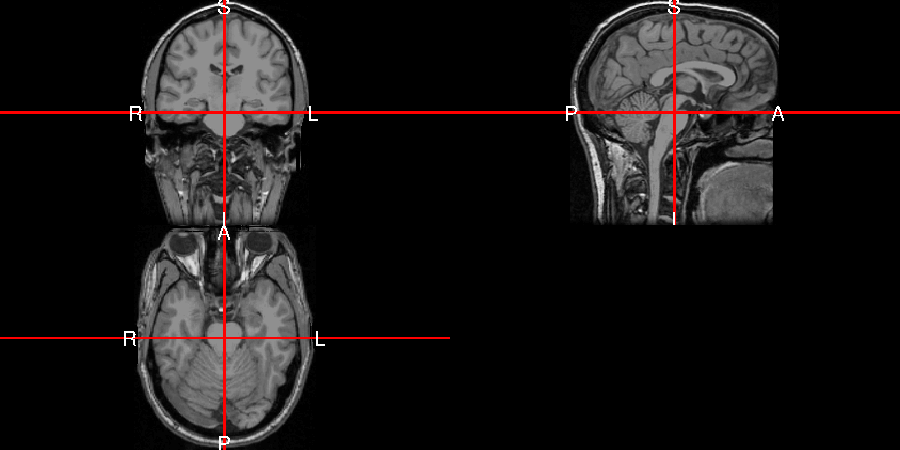
\includegraphics{Freesurfer_files/figure-latex/mri_plot2-1} \caption[Plot of T1-weighted image from bert subject in Freesurfer after re-orientation to RPI orientation]{Plot of T1-weighted image from bert subject in Freesurfer after re-orientation to RPI orientation.  Note, the letters denote the orientation of right/left (R/L), posterior/anterior (P/A), inferior/superior (I/S). }\label{fig:mri_plot2}
\end{figure}
\end{Schunk}

The result is in figure \ref{fig:mri_plot2}, which changes the views in
reference to which panel they are located and matches the orientation
markers assumed by \code{ortho2}.

\subsection{\texorpdfstring{Bias-field correction: the
\code{nu\_correct}
function}{Bias-field correction: the  function}}\label{bias-field-correction-the-function}

MRI images typically exhibit good contrast between soft tissue classes,
but intensity inhomogeneities in the radio frequency field can cause
differences in the ranges of tissue types at different spatial locations
(e.g.~top versus bottom of the brain). These
inhomogeneities/non-uniformities can cause problems with algorithms
based on histograms, quantiles, or raw intensities
\citep{zhang_segmentation_2001}. Therefore, correction for image
inhomogeneities is a crucial step in many analyses. The Freesurfer
function \code{nu\_correct} performs the non-uniformity correction by
\citet{sled_nonparametric_1998} and the \pkg{freesurfer} function of the
same name will run the correction and return an image.

The Freesurfer \code{nu\_correct} function requires a MINC format
(\url{http://www.bic.mni.mcgill.ca/ServicesSoftware/MINC}). For this to
work, you can convert the \code{nifti} object to a MINC file using
\code{nii2mnc}:

\begin{Schunk}
\begin{Sinput}
mnc = nii2mnc(reoriented_img)
print(mnc)
\end{Sinput}
\begin{Soutput}
[1] "/var/folders/1s/wrtqcpxn685_zk570bnx9_rr0000gr/T//RtmpfoWZn1/file163571751571f.mnc"
\end{Soutput}
\end{Schunk}

We can pass this MINC file into the \pkg{freesurfer} \code{nu\_correct}
function, which will run the correction and then convert the output MNC
to a NIfTI object.

\begin{Schunk}
\begin{Sinput}
nu_from_mnc = nu_correct(file = mnc)
class(nu_from_mnc)
\end{Sinput}
\end{Schunk}

\begin{Schunk}
\begin{Soutput}
[1] "nifti"
attr(,"package")
[1] "oro.nifti"
\end{Soutput}
\end{Schunk}

We see that the results are indeed \code{nifti} objects. We can plot the
estimated bias field (log-transformed for display purposes) side-by-side
the image to view which areas had been differentially corrected (Figure
\ref{fig:nu_correct_plot}).

\begin{Schunk}
\begin{figure}
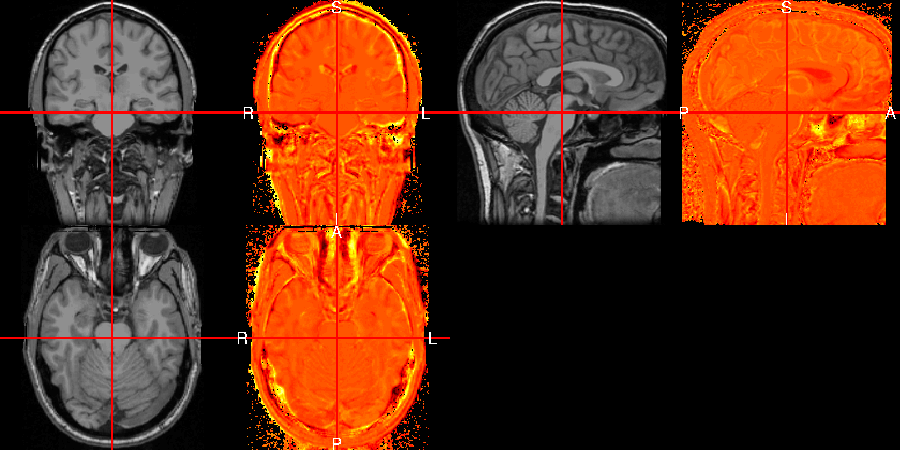
\includegraphics{Freesurfer_files/figure-latex/nu_correct_plot-1} \caption[Inhomogeneity-corrected image output from Freesurfer \code{nu\_correct} command and the estimated log bias-field]{Inhomogeneity-corrected image output from Freesurfer \code{nu\_correct} command and the estimated log bias-field.}\label{fig:nu_correct_plot}
\end{figure}
\end{Schunk}

In addition to the \code{readmgz} and \code{readmgh} functions above, we
have a \code{readmnc} wrapper function for reading in MINC files, after
conversion to NIfTI files. If you pass in a \code{nifti} object in
directly into \texttt{nu\_correct}, the function will automatically
convert any NIfTI input files, and then run the correction (shown
below). We can also pass in a mask (generated from above) to run the
correction only the areas of the brain.

\begin{Schunk}
\begin{Sinput}
nu_masked = nu_correct(file = reoriented_img, mask = mask)
class(nu_masked)
\end{Sinput}
\begin{Soutput}
[1] "nifti"
attr(,"package")
[1] "oro.nifti"
\end{Soutput}
\end{Schunk}

Overall, this correction is a way to make the intensities of the brain
more homogeneous spatially. This method is different from that
implemented in FSL \citep{jenkinson_fsl_2012} (and therefore
\pkg{fslr}), so it provides an alternative method to the R user than
currently available.

\subsection{\texorpdfstring{Brain extraction: the \code{mri\_watershed}
function}{Brain extraction: the  function}}\label{brain-extraction-the-function}

The \code{mri\_watershed} function will segment the brain from the
remainder of the image, such as extra-cranial tissues. Other imaging
software in R have implemented the watershed algorithm, such as
\BIOpkg{EBImage} \citep{EBImage}. These methods have not been directly
adapted for MRI nor specifically for brain extraction. In
\pkg{freesurfer}, we can pass in the \code{nifti} object and the output
is a brain-extracted \code{nifti} object.

\begin{Schunk}
\begin{Sinput}
ss = mri_watershed(img)
ortho2(ss, mask = ss)
\end{Sinput}
\end{Schunk}

\begin{Schunk}
\begin{figure}
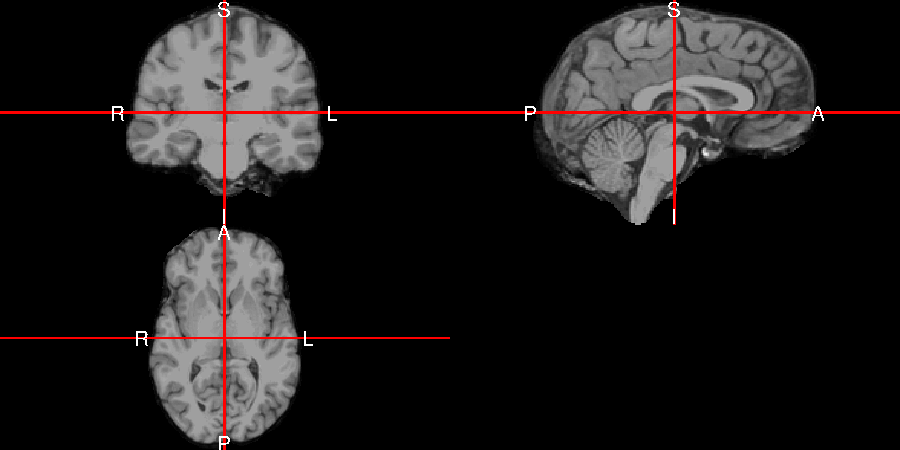
\includegraphics{Freesurfer_files/figure-latex/watershed_plot-1} \caption[Brain-extracted image after using Freesurfer \code{mri\_watershed} algorithm]{Brain-extracted image after using Freesurfer \code{mri\_watershed} algorithm.  We see that the areas outside of the brain have been removed from the image.}\label{fig:watershed_plot}
\end{figure}
\end{Schunk}

The result is in figure \ref{fig:watershed_plot}, where we see areas of
the skull, eyes, face, and other areas of the image are removed. We do
see some areas remain that may be part of some of the membranes between
the brain and the skull, but this looks like an adequate brain
extraction for most analyses.

As the result in a \code{nifti} object, we can create a mask by standard
logical operations for arrays. As MRI scans are typically
positive-valued, the positive areas of the image are the ``brain'':

\begin{Schunk}
\begin{Sinput}
mask = ss > 0
\end{Sinput}
\end{Schunk}

We can then use this mask to perform operations on the image, such as
subsetting.

\subsection{Segmentations of Brain
Structures}\label{segmentations-of-brain-structures}

Freesurfer is commonly used to segment cortical and subcortical
structures of the brain. We can visualize images of these segmentations,
which are located in the ``mri'' folder. We will choose the colors based
on the Freesurfer look up table (LUT), which values can be explored at
\url{https://surfer.nmr.mgh.harvard.edu/fswiki/FsTutorial/AnatomicalROI/FreeSurferColorLUT}.
This look up table provides a label for each structure and the color
associated with it:

\begin{Schunk}
\begin{Sinput}
head(freesurfer::fs_lut, 3)
\end{Sinput}
\begin{Soutput}
  index                      label   R   G   B A
1     0                    Unknown   0   0   0 0
2     1     Left-Cerebral-Exterior  70 130 180 0
3     2 Left-Cerebral-White-Matter 245 245 245 0
\end{Soutput}
\end{Schunk}

This object is included in \pkg{freesurfer} and denotes the indices,
labels, and color representation of the structure. We note that the
alpha channel is set to \(0\) for all regions of interest, so we will
not use it in the calculation of the colors from RGB space. This LUT
allows visualizations produced in R to be consistent with those from
Freesurfer.\\

\begin{Schunk}
\begin{Sinput}
seg_file = file = file.path(fs_subj_dir(), "bert", "mri", "aseg.mgz")
seg = readmgz(seg_file)
breaks = c(-1, fs_lut$index)
colors = rgb(fs_lut$R, fs_lut$G, fs_lut$B, alpha = 255/2, maxColorValue = 255)
ortho2(ss, seg, col.y = colors, ybreaks = breaks)
\end{Sinput}
\end{Schunk}

\begin{Schunk}
\begin{figure}
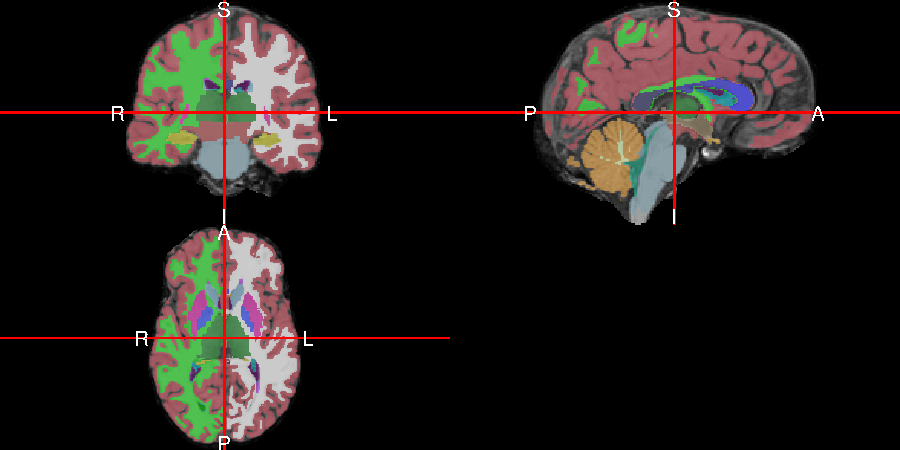
\includegraphics{Freesurfer_files/figure-latex/seg_file-1} \caption[Overlay of segmentation from Freesurfer \code{recon-all} command]{Overlay of segmentation from Freesurfer \code{recon-all} command.  }\label{fig:seg_file}
\end{figure}
\end{Schunk}

Note above that the number of breaks must be one larger than the number
of colors and the indices start at zero, so we add an additional element
to the indices. The result in figure \ref{fig:seg_file} shows the image
with colors overlaid.

\subsection{Reading in anatomical statistics for brain
structures}\label{reading-in-anatomical-statistics-for-brain-structures}

We have explored the spatial results in the brain images, but not the
quantitative information about the brain and sub-structures are
available from Freesurfer output. The ``aseg.stats'' in the ``stats''
folder for subject bert corresponds to measures and statistics from the
anatomical segmentation. The \code{read\_aseg\_stats} function reads
this corresponding file and creates a list of 2 different
\code{data.frame}s:

\begin{Schunk}
\begin{Sinput}
file = file.path(fs_subj_dir(), "bert", "stats", "aseg.stats")
out = read_aseg_stats(file)
names(out)
\end{Sinput}
\begin{Soutput}
[1] "measures"   "structures"
\end{Soutput}
\end{Schunk}

The \code{measures} element corresponds to global measurements of the
brain (e.g.~volume of the brain) as well as measures of gross anatomical
structures (e.g.~gray matter).

\begin{Schunk}
\begin{Sinput}
head(out$measures[, c("meaning", "value", "units")], n = 3)
\end{Sinput}
\begin{Soutput}
                                                 meaning          value
1                              brain segmentation volume 1193318.000000
2           brain segmentation volume without ventricles 1174082.000000
3 brain segmentation volume without ventricles from surf 1173867.217735
  units
1  mm^3
2  mm^3
3  mm^3
\end{Soutput}
\end{Schunk}

In some imaging analyses, comparing at these large measures of brain volume over time or across groups are of interest.  Alternatively, the \code{structures} element corresponds to a set of measures and statistics for a set of fixed anatomical structures.

\begin{Schunk}
\begin{Sinput}
head(out$structures, n = 3)
\end{Sinput}
\begin{Soutput}
  Index SegId NVoxels Volume_mm3                   StructName normMean
1     1     4    6563     6562.6       Left-Lateral-Ventricle  36.0959
2     2     5     228      228.3            Left-Inf-Lat-Vent  54.8842
3     3     7   15708    15708.2 Left-Cerebellum-White-Matter  92.7562
  normStdDev normMin normMax normRange
1    12.2771      16      91        75
2    10.7839      22      87        65
3     5.5123      40     107        67
\end{Soutput}
\end{Schunk}

Similarly with global measures, these structure-specific measures are
used in analysis. For example, measuring differences in hippocampus
volumes across patients with Alzheimer's disease and those without.
Moreover, a large deviation in volume, globally or locally, for a
specific subject may indicate atrophy of a structure or an indication of
a segmentation error.

\subsection{\texorpdfstring{Converting surfaces using
\code{mris\_convert}}{Converting surfaces using }}\label{converting-surfaces-using}

Freesurfer includes seegmentations of different surfaces of the brain
alongside the volumetric segmentations above. As the \code{mri\_convert}
function provides a tool to convert image volumes to a series of output
formats, the \code{mris\_convert} (note the ``s'') allows users to
convert between image surface formats. These surfaces usually store sets
of vertices and faces to be plotted in 3 dimensions. \pkg{freesurfer}
has implemented \code{mris\_convert} (with a function of the same name)
as well as functions to convert surfaces from Freesurfer to a set of
triangles in R, such as \texttt{surface\_to\_triangles}. We will read in
the left and right side of the pial surface of the brain and display the
surface using \CRANpkg{rgl} \citep{rgl}.

\begin{Schunk}
\begin{Sinput}
right_file = file.path(fs_subj_dir(), 
                   "bert", "surf", "rh.pial")
right_triangles = surface_to_triangles(infile = right_file)
left_file = file.path(fs_subj_dir(), 
                   "bert", "surf", "lh.pial")
left_triangles = surface_to_triangles(infile = left_file) 
rgl::rgl.open()
rgl::rgl.triangles(right_triangles, 
                   color = rainbow(nrow(right_triangles)))
rgl::rgl.triangles(left_triangles, 
                   color = rainbow(nrow(left_triangles)))
\end{Sinput}
\end{Schunk}

\begin{figure}
\centering
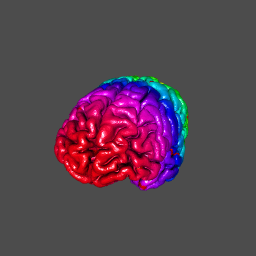
\includegraphics{Freesurfer_files/figure-latex/rgl_plot_out.png}
\caption{Pial surface from bert subject in Freesurfer rendered using
\pkg{rgl}.}
\end{figure}

Thus, we can read in the output images, surfaces, and the tables of
output metrics from Freesurfer.

\subsection{Additional Features}\label{additional-features}

For the initial release, we did not implement a method to read the
annotation files and other surface-based files that Freesurfer uses.
Reading in these files are planned for a future release and may work
with the functions described above. Freesurfer can also analyze
diffusion tensor imaging data and some of the functions have been
adapted for \pkg{freesurfer} but have not been thoroughly tested.

\section{Conclusion}\label{conclusion}

The neuroimaging community has developed a large collection of tools for
image processing and analysis. These tools have additional functionality
that is not present in R, such as the surface-based registration and
processing Freesurfer provides. We have provided a similar incorporation
of tools from FSL to R in the \pkg{fslr} package and have repeated the
effort for Freesurfer with the \pkg{freesurfer} package to bridge this
gap and provide R users functions from Freesurfer.

There has been an increasing popularity of similar interfacing of tools
within the Python community such as Nipype
\citep{gorgolewski_nipype:_2011}
(\url{https://qa.debian.org/popcon.php?package=nipype}). As many users
of R may not have experience with Python or bash scripting, we believe
\pkg{freesurfer} provides a lower threshold for use in the R community.

Lowering this threshold is important because it allows more R users to
control all aspects of image analysis from raw image processing to final
statistical analysis. Interfacing R with existing, powerful software
provides R users more functionality and a additional support community,
which would not be available if the functions were rewritten in R.
Although having an external software dependency may be disadvantage to R
users, the software used benefits from the years of previous testing.
Most importantly, as \pkg{freesurfer} is based on the R framework, all
the benefits of using R are available, such as dynamic documents, Shiny
applications, customized figures, and state-of-the-art statistical
methods. This added functionality affords the neuroimaging and R
communities the ability to have analysis in one framework while
borrowing the strengths of both.

\section{Reproducibility}\label{reproducibility}

This paper was generated using the \CRANpkg{rticles} package
\citep{rticles}. All necessary code to generate this report is located
at: \url{https://github.com/muschellij2/fs_paper}.

\bibliography{RJreferences}

\section{Supplemental Material}\label{supplemental-material}

\subsection{Label files}\label{label-files}

Although we have not thoroughly tested reading in a label file from
Freesurfer, we have provided the \code{read\_fs\_label} function. Here
we will read a label file for the left hemisphere cortex:

\begin{Schunk}
\begin{Sinput}
file = file.path(fs_subj_dir(), "bert", "label", "lh.cortex.label")
out = read_fs_label(file)
head(out)
\end{Sinput}
\begin{Soutput}
  vertex_num r_coord  a_coord s_coord        value
1          0 -12.882 -102.449  -9.782 0.0000000000
2          1 -13.331 -102.518  -9.829 0.0000000000
3          2 -13.637 -102.514 -10.077 0.0000000000
4          3 -13.031 -102.596 -10.024 0.0000000000
5          4 -13.331 -102.510 -10.254 0.0000000000
6          5 -13.610 -102.483 -10.295 0.0000000000
\end{Soutput}
\end{Schunk}

The coordinates are mostly used in these files, not the value assigned
(in this case all zeroes). These files can be used for registration as
well. Overall, we have provided a reader for users, but have not used
them in our research and therefore have not tested them extensively to
discuss them further.

\address{%
John Muschelli\\
Johns Hopkins Bloomberg School of Public Health\\
Department of Biostatistics\\ 615 N Wolfe St, Baltimore, MD, 21205\\
}
\href{mailto:jmuschel@jhsph.edu}{\nolinkurl{jmuschel@jhsph.edu}}

\address{%
Elizabeth M. Sweeney\\
Rice University\\
Department of Statistics\\ 6100 Main St, Duncan Hall, Houston, TX, 77005\\
}
\href{mailto:ems15@rice.edu}{\nolinkurl{ems15@rice.edu}}

\address{%
Ciprian M. Crainiceanu\\
Johns Hopkins Bloomberg School of Public Health\\
Department of Biostatistics\\ 615 N Wolfe St, Baltimore, MD, 21205\\
}
\href{mailto:ccraini1@jhu.edu}{\nolinkurl{ccraini1@jhu.edu}}

